\section{Model of the Interconnect}
\label{sec:model:bus}
This section presents the automata corresponding to the interconnect. As the
split-transaction bus architectures are the target, it is unsurprising that the
model of the interconnect finds itself also split into two parts: a query bus,
and a data bus.

\subsection{Data Bus}
\begin{figure}[hbt!]
\begin{center}
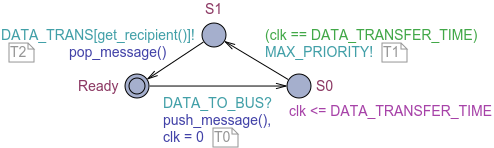
\includegraphics[width=0.6\textwidth]{\chapterdirectory/figure/DataBus.pdf}
\end{center}
\caption{Automaton for the Data Bus}
\label{fig:UPPAAL:DataBus}
\end{figure}

Figure~\ref{fig:UPPAAL:DataBus} shows the automaton used for the data bus.  It
uses a single variable and a single clock:
\paragraph{Clocks \& Variables for Data Bus}
\begin{itemize}
\item
   \lstinline!clk! is a clock controlling the time the data bus stays
   inactive before transmitting a data message to its target.
\item
   \lstinline!msg! is a message to communicate.
\end{itemize}
%\end{varandclocks}

As it does not have need for an initialization transition, the \texttt{Ready}
location is the initial one.

\paragraph{Transitions for Data Bus}
\begin{description}
\item[$\texttt{Ready} \automatatransitiontrace{T_{0}}{} S_0$]
   Upon any automaton synchronizing on the \textbf{DATA\_TO\_BUS} channel,
   the message in the information sharing global variable is copied to
   \lstinline!msg! and \lstinline!clk! is set to zero, as the data transfer
   waiting period starts.

\item[$S_0 \automatatransitiontrace{T_{1}}{} S_1$]
   As soon as the \lstinline!DATA_TRANSFER_TIME! period is elapsed, the
   automaton moves to the $S_1$ in order to synchronize with the message's
   target automaton.

\item[$S_1 \automatatransitiontrace{T_{2}}{} \texttt{Ready}$]
   By synchronizing on the \textbf{DATA\_TRANS} sub-channel that corresponds to
   the ID of the recipient of \lstinline!msg!, the data bus automaton stores
   \lstinline!msg! in the information sharing global variable so that the other
   automaton is able to receive it. Once this is done, the data bus automaton
   becomes once again available for a new data message transfer.
\end{description}

\subsection{Query Bus}
\begin{figure}[hbt!]
\begin{center}
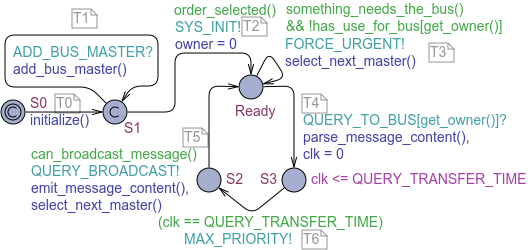
\includegraphics[width=0.7\textwidth]{\chapterdirectory/figure/QueryBus.pdf}
\end{center}
\caption{Automaton for the Query Bus}
\label{fig:UPPAAL:QueryBus}
\end{figure}
Figure~\ref{fig:UPPAAL:QueryBus} shows the automaton used for the query bus. It
is considerably more complex than the data one, as it features an access
policy. The access policy it models is a simple round-robin one, with the
order being defined once prior the \textbf{SYS\_INIT} signal being emitted,
then followed during the whole execution. The round-robin policy is not strict:
if the next bus user in line does not need to use the bus, its turn is skipped.

The query bus automaton has the following clock and variables:
\paragraph{Clocks \& Variables for Query Bus}
\begin{itemize}
\item
   \lstinline!clk! is a clock controlling the time the query bus stays inactive
   before broadcasting a new query.
\item \lstinline!msg! is a copy of the message to broadcast.
\item
   \lstinline!bus_master_order! is an array indicating the order in which
   components can use the bus. It stores component IDs.
\item
   \lstinline!owner! is the index for \lstinline!bus_master_order!
   corresponding to the current bus owner.
\end{itemize}
%\end{varandclocks}

The query bus has a fairly complex initialization procedure, as it needs to
define its access policy before the model is fully initialized. It starts in
the $S_0$ location.

\paragraph{Transitions for Query Bus}
\begin{description}
\item[$S_0 \automatatransitiontrace{T_{0}}{} S_1$]
   The query bus automaton initializes many global variables in this transition:
   the default value of the information passing global variable is set; the
   \lstinline!has_use_for_bus! array is initialized with \lstinline!false! in
   every slot; and the \lstinline!is_ready_for_bus! array is initialized with
   \lstinline!true! in every slot.

   The local variable \lstinline!owner! is set to zero. The
   \lstinline!bus_master_order! array is filled with the component ID of the
   query bus, a sane value to use as default.

   Once all these variables have been set to sane defaults, the query bus is
   ready to register bus masters.

\item[$S_1 \automatatransitiontrace{T_{1}}{} S_1$]
   By synchronizing on the \textbf{ADD\_BUS\_MASTER} channel, other automata
   (namely cache automata), can register as bus master. There is no order
   defined for these synchronizations to take place: automata seeking to be
   added as bus master are all attempting to do so simultaneously. Since this is
   not a broadcast channel, a non-deterministic order is chosen and will be
   followed for the rest of the automata's execution.

   This transition copies the component ID of the emitter of the message in the
   information transmission global variable, and stores it in the next available
   \lstinline!bus_master_order! slot. The \lstinline!owner! variable is used to
   keep track of how many slots have been used so far.

\item[$S_1 \automatatransitiontrace{T_{2}}{} \texttt{Ready}$]
   Completion of the bus master selection is detected by seeing that the number
   of slots allocated in \lstinline!bus_master_order!, as indicated by
   \lstinline!owner!, has reached \lstinline!CORE_COUNT!.

   Once this happens, \lstinline!owner! is set back to zero and the
   \textbf{SYS\_INIT} broadcast occurs, leading all other automata to perform
   their final initialization step. Likewise, the query bus automaton becomes
   ready to accept incoming queries.

\item[$\texttt{Ready} \automatatransitiontrace{T_{4}}{} S_3$]
   The query bus awaits an incoming query from its current bus owner
   (\lstinline!bus_master_order[owner]!). Thus, that component's automaton
   has to synchronize on its dedicated \textbf{QUERY\_TO\_BUS} sub-channel.
   This synchronization leads the query bus to copy the content of the
   information sharing global variable to \lstinline!msg!, set \lstinline!clk!
   to zero and start waiting for the query transfer time.

\item[$S_3 \automatatransitiontrace{T_{6}}{} S_2$]
   Once the query bus has stayed inactive in $S_3$ for a duration of
   \lstinline!QUERY\_TRANSFER\_TIME!, it immediately moves to the $S_2$ location
   in order to broadcast the query held in \lstinline!msg!.

\item[$S_2 \automatatransitiontrace{T_{5}}{} \texttt{Ready}$]
   To be able to perform this transition without risking the query not reaching
   one of the automata that needs to receive it, the guard ensures that all
   slots of \lstinline!is_ready_for_bus! hold \lstinline!true!.

   As soon as this is the case, the content of the query in \lstinline!msg! is
   put in the information sharing global variable and broadcasts on the
   \textbf{QUERY\_BROADCAST} channel.

   During this transition, the \lstinline!owner! variable is incremented by one,
   or set back to zero if it had reached the end of the
   \lstinline!bus_master_order! array. The query bus is then once again ready to
   accept a query, this time from the new bus master.

\item[$\texttt{Ready} \automatatransitiontrace{T_{5}}{} \texttt{Ready}$]
   But if the current bus master has not set \lstinline!true! in its dedicated
   slot in \lstinline!has_use_for_bus!, yet some other component has set
   \lstinline!true! in their dedicated slot, the query bus uses this transition
   to increment the \lstinline!owner! variable so that it points to the next
   bus owner. Since the destination location is unchanged, this process is
   repeated until a component with a need for the bus is chosen as bus master.

   Note that ensuring that at least one component needs the query bus is
   crucial, as the transition would otherwise be activated ad infinitum once all
   programs have completed.
\end{description}
